% =========================================================================== %

\begin{frame}[t,plain]
\titlepage
\end{frame}

% =========================================================================== %

\begin{frame}{Recap}
%
\begin{columns}[T]
\column{.5\linewidth}
\textbf{MatPlotLib}
\begin{itemize}
\item Commands \texttt{plt.plot(X, Y)} and \texttt{plt.show()}
\item \texttt{plt.bar}, \texttt{plt.scatter}, \texttt{plt.quiver}, ...
\item Millions of optional arguments
\item Plot-Objekts \texttt{figure} and \texttt{axis}
\item In doubt: Look it up on \url{https://matplotlib.org/} or in the lecture notes
\end{itemize}
%
\column{.5\linewidth}
\textbf{NumPy}
\begin{itemize}
\item Central element: \texttt{np.ndarray}
\item Componentwise operations
\item Create from Python \texttt{list}s or using dedicated functions
\item Proper math library for fast vectorized operations
\item Proper commands for reduction (\eg \texttt{np.sum})
\end{itemize}

\end{columns}
%
\begin{center}
	\emph{Any Questions?}
\end{center}
%
\end{frame}

% =========================================================================== %

\begin{frame}[fragile]
%
\begin{tcbraster}[raster columns=2,
                  raster equal height,
                  nobeforeafter,
                  raster column skip=0.5cm]
\begin{codebox}[Beispiel: Title goes here]
\begin{minted}[fontsize=\scriptsize, linenos]{python}
foo
\end{minted}
\end{codebox}
%
\begin{codebox}[Beispiel: Title goes here]
\begin{minted}[fontsize=\scriptsize, linenos]{python}
bar
\end{minted}
\end{codebox}
\end{tcbraster}
%
\end{frame}

% =========================================================================== %

\begin{frame}[fragile]{Plan for Today}
%
\begin{itemize}
\item Some Physics: 
	\begin{itemize}
	\item Spin lattice and magnetism
	\item Energy
	\item Boltzmann distribution
	\end{itemize}
\item Representing reality in code
	\begin{itemize}
	\item List of properties and questions
	\item Choosing apt data structures
	\item First methods
	\end{itemize}
\item Metropolis algorithm
	\begin{itemize}
	\item Bit configuration spaces and Monte Carlo methods
	\item Metropolis algorithm \enquote{for humans}
	\item Metropolis algorithm in Python
	\end{itemize}
\end{itemize}
%
\end{frame}

% =========================================================================== %

\begin{frame}{Physics: Spin Lattice}
%
\begin{columns}[T]
\column{.5\linewidth}
\begin{itemize}
\item Picture: atoms as little bar magnets
\item Freely rotatable in space
	\begin{itemize}
	\item Simplification: only two orientations
	\item either: north pole \enquote{up}
	\item or: Nordpol \enquote{down}
	\end{itemize}
\item Magnetic fields sum up
	\begin{itemize}
	\item Parallel alignments reinforce one another
	\item Antiparalellel alignments cancel out
	\end{itemize}
\item Representation of solid: grid of bar magnets
\end{itemize}
%
\column{.5\linewidth}
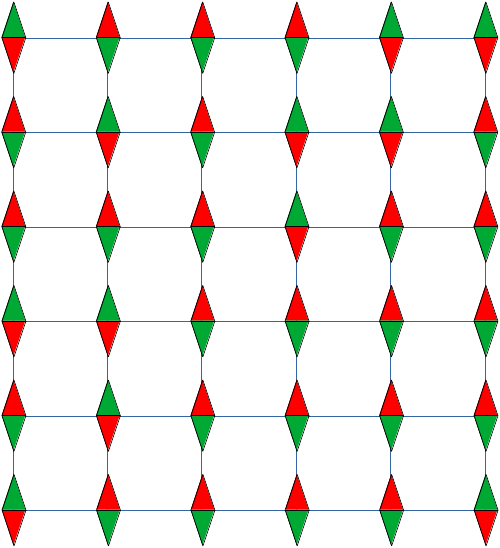
\includegraphics[width=.7\linewidth]{./gfx/spinLattice}
\end{columns}
%
\end{frame}

% =========================================================================== %\\

\begin{frame}{Physics: Total Magnetization and Energy in the Lattice}
%
\begin{columns}[T]
\column{.5\linewidth}
\begin{itemize}
\item Total magnetization
	\begin{itemize}
	\item \enquote{How strong is the magnetic field of the entire lattice?}
	\item {}[Number of spin up atoms] minus [number of spin down atoms]
	 \end{itemize} 
\item Total lattice energy
	\begin{itemize}
	\item Magnets attract or repell each other
	\item There is an \enquote{energy cost} to bring equal poles together
	\item Depends on distance
	\item Simplification: Only next neighbours relevant
	\end{itemize}
\end{itemize}
%
\column{.5\linewidth}
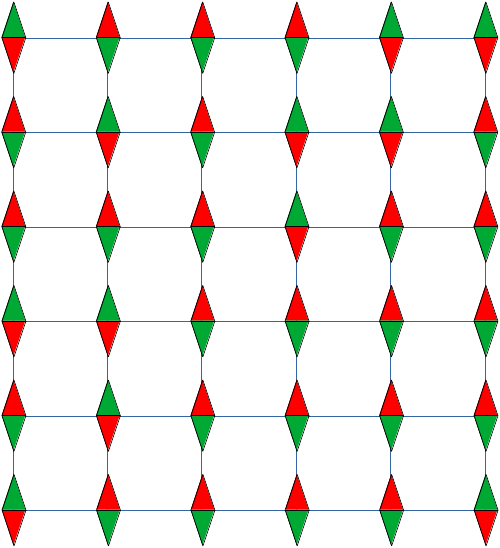
\includegraphics[width=.7\linewidth]{./gfx/spinLattice}
\end{columns}
%
\end{frame}

% =========================================================================== %\\

\begin{frame}{Physics: Magnetization Density and Lattice Energy in Equations}
%
\begin{itemize}
\item Represent each magnet by a number $+1$ or $-1$
\item Lattice in its entirety: table (matrix): $G = \left( g_{ij} \right)$
\item Magnetization density
	\[ M = \frac{1}{V} \sum_{i, j} g_{ij} \qquad \text{where } V: \text{\enquote{Volume}, number of atoms} \]
\item Energy
	\begin{itemize}
	\item Coupling constant $J$
	\item For each neighbour with \emph{parallel} spin: gain energy $J$
	\item For each neighbour with \emph{antiparallelen} spin: energy cost $J$
	\item If $i$ is neighbour of $j$, then $j$ is neighbour of $i$, too. But energy cost only once!
	\item 
		\begin{align*}
			E &= -\frac{J}{2V} \sum_x \sum_{y: y \text{ is neighbour of }x} g_x \cdot g_y 
			  = -\frac{J}{2V} \sum_{<x, y>} g_x \cdot g_y
		\end{align*}			
	\item Attention: $x, y$ are \emph{coordinates}; $x$ \enquote{contains} row- \emph{and} column ID
	\end{itemize}
\end{itemize}
%
\end{frame}

% =========================================================================== %

\begin{frame}{Physics: Expectation Value}
%
\begin{itemize}
\item A priori: Spins independent from one another
\item For $V = L \cdot L$ lattice points: $2^V$ possible arrangements
\item Each arrangement: different energy
\item Not all arrangements equally likely!
\item Real world:
	\begin{itemize}
	\item Energy of an object is subject to fluctuations
	\item Thus: any state is possible
	\end{itemize}
\item Probability to realize a particular state depends on its energy! $p = p(E)$
\item Expectation value for magnetization:
	\[ <M> ~ = \sum_{\text{state } G} p[E(G)] \cdot M(G) \]
\end{itemize}
%
\end{frame}

% =========================================================================== %

\begin{frame}{Physics: Boltzmann Distribution}
%
Boltzmann distribution:
\[ p(E) = \frac
	{\exp( -\frac{E}{k_B T} )}
	{\sum_\mathcal{E} \exp( -\frac{\mathcal{E}}{k_B T} )}
\]

Where:
\begin{itemize}
\item $T$: Temperature in Kelvin
\item $k_B$: Boltzmann constant
\end{itemize}

Thus:
\begin{itemize}
\item \emph{In prinziple} magnetization for eavery temperature can be computed
\item \emph{In practice} too time intensive
\end{itemize}

Outlook:
\begin{itemize}
\item Metropolis algorithm circumvents this problem
\end{itemize}
%
\end{frame}

% =========================================================================== %

\begin{frame}{Programming: From Reality to Code}
%
We need:
\begin{itemize}
\item Given: Temperature
\item A lattice
	\begin{itemize}
	\item Comprising of atoms
	\item Atoms have property \emph{spin}: $+1$ or $-1$
	\item Property: magnetization
	\item Property: total energy
	\item Relation: \enquote{is neighbour of}
	\item Given: initial state
	\end{itemize}
\item Probability to realize a particular state of the lattice
\end{itemize}
%
\end{frame}

% =========================================================================== %

\begin{frame}[fragile]{Programming: Ordering our Analysis}
%
\begin{itemize}
\item Temperature: only important once we get to probabilities
\item Lattice: \enquote{feels like an object} \Thus class
	\begin{itemize}
	\item State $G$: Collection of spins \Thus Array-like (\inPy{list}, NumPy-Array, ...)
		\begin{itemize}
		\item Equal data types ($+1$ or $-1$)
		\item Filled table
		\item[\Thus] NumPy-Array; data type \texttt{np.int64}
		\item Thus, implicitly \emph{Adressing} atoms by their indices
		\end{itemize}
	\item \enquote{Questions to the lattice}: magnetization and energy
		\begin{itemize}
		\item Can be computed from $G$ and $J$ alone
		\item[\Thus] Methods
		\end{itemize}
	\item Neighbour-relation
		\begin{itemize}
		\item Could be computed from coordinates and lattice dimension
		\item But: Needed very frequently
		\item Alternative: Compute once, store in memory
		\item[\Thus] Second NumPy-Array
		\end{itemize}
	\end{itemize}
\end{itemize}
%
\end{frame}

% =========================================================================== %

\begin{frame}{Programming: Select Subproblems}
%
\begin{itemize}
\item We see: our description \enquote{explodes} 
	\begin{itemize}
	\item Already jotted down a lot of notes
	\item Neighbourhood relation not yet fully described
	\item No thoughs at all for coding probabilites
	\end{itemize}
\item But: already quite some concrete thoughs on representation of the lattice
\item[\Thus] Select concrete results, set back the rest
\end{itemize}
%
\end{frame}

% =========================================================================== %

\begin{frame}[fragile]{Programming: class \texttt{Grid} -- first concept}
%
\begin{tcolorbox}[title=class \texttt{Grid}]
\begin{itemize}
\item Class attributes
	\begin{itemize}
	\item None (If we regard two lattices in the same program, they will have nothing in common)
	\end{itemize}
\item Instance attributes
	\begin{itemize}
	\item NumPy-Array \texttt{spins}
	\item \inPy{int L}: width of the lattice (not indispensible, but \enquote{more comfortable})
	\item \inPy{float J}: coupling constant (necessary for computing the energy)
	\end{itemize}
\item Methoden
	\begin{itemize}
	\item \inPy{__init__(self, L, J, ??)} (maybe additional parameters): prepares a lattice in some \emph{initial state}
	\item \texttt{getMagnetization(self)} (no further parameters)
	\item \texttt{getEnergy(self)} (no further parameters)
	\end{itemize}
\end{itemize}
\end{tcolorbox}
%
\end{frame}

% =========================================================================== %

\begin{frame}[fragile]{Programming: class \texttt{Grid} -- first code}
%
\begin{codebox}
\begin{minted}[linenos, fontsize=\scriptsize]{python3}
import numpy as np

class Grid :
    def __init__ (self, L, J = 1) :
        self.L     = L
        self.J     = J
        self.spins = np.ones(shape = (L, L), dtype=np.int64)

g = Grid(5)
print(g.spins)
\end{minted}
\end{codebox}
%
\begin{hintbox}[Answer open questions as simply as possible]
The \emph{initial state} wasn't covered in our regards so far. In such a case: start with a simple fill-in, like here: \texttt{np.ones}
\end{hintbox}
%
\end{frame}

% =========================================================================== %

\begin{frame}[fragile]{Retrofit the forgotten part}
%
\begin{itemize}
\item What does \emph{initial state} mean?
	\begin{itemize}
	\item Example: probability for any atom to be spin up
	\item[\Thus] \inPy{float}-argument \texttt{p}: probability
	\end{itemize}
\item Deduce \emph{effects} from this amendment
	\begin{itemize}
	\item Spins now random
	\item[\Thus] no new attributes to the class
	\item[\Thus] \texttt{np.ones} no longer sufficient
	\end{itemize}
\item Include new effect in the method
	\begin{itemize}
	\item Tasks performed by a method should remain simple
	\item \enquote{One thought -- one method}. Rarely more than 20 lines per function/method
	\item New method: pick atoms at random and flip their spin
	\end{itemize}
\end{itemize}
%
\end{frame}

% =========================================================================== %

\begin{frame}[fragile]
%
\begin{codebox}
\begin{minted}[linenos, fontsize=\scriptsize]{python3}
import numpy as np

class Grid :
    def __init__ (self, L, J = 1, p = None) :
        self.L     = L
        self.J     = J
        self.spins = np.ones(shape = (L, L), dtype=np.int64)
        
        if p : self.shake(p)
        
    def shake (self, p = 0.5) :
        mask = np.random.uniform(size = (self.L, self.L)) < p
        self.spins[mask] *= -1

g = Grid(5, 1, 0.5)
print(g.spins)
\end{minted}
\end{codebox}
%
\end{frame}

% =========================================================================== %

\begin{frame}[fragile]{New methods}
%
\begin{tcbraster}[raster columns=2,
                  raster equal height,
                  nobeforeafter,
                  raster column skip=0.5cm]
\begin{codebox}[First planned method]
\begin{minted}[linenos, fontsize=\scriptsize]{python3}
import numpy as np

class Grid :
    # as before
    
    def magnetization (self) :
        return np.sum(self.spins) / \
               self.L ** 2
    
    def energy (self) :
        # ???
        pass

g = Grid(5, 1, 0.5)
print(g.spins)
print(g.magnetization())
\end{minted}
\end{codebox}
%
\begin{cmdbox}[Output]
\begin{minted}[fontsize=\scriptsize]{text}

[[ 1 -1  1 -1 -1]
 [-1  1  1 -1 -1]
 [ 1  1  1 -1  1]
 [ 1  1 -1 -1  1]
 [-1 -1 -1 -1 -1]]
-0.12
\end{minted}
\end{cmdbox}
\end{tcbraster}
%
\end{frame}

% =========================================================================== %

\begin{frame}[fragile]{Neighbour Lists}
%
\begin{itemize}
\item Already discussed: trade memory for processor time
\item Analogous thoughts to construction of the lattice
	\begin{itemize}
	\item List of coordinates
	\item Always same data type, completely filled table
	\item[\Thus] NumPy-Array
	\item \enquote{Table with \inPy{tuple}s as entries} (4 neighbours with row and column)
	\end{itemize}
\item Put it into the code...
	\begin{itemize}
	\item ... as a proper method ...
	\item ... called by \inPy{__init__}
	\end{itemize}
\item Special case: boundaries?
	\begin{itemize}
	\item Different possibilities
	\item Most common, most simple approach: \emph{cyclical boundary conditions}: left boundary connected to the right, upper boundary connected to the bottom one
	\item Alternatively: leave empty, modulus neighbourhood, ...
	\end{itemize}
\end{itemize}
%
\end{frame}

% =========================================================================== %

\begin{frame}[fragile]
%
\begin{codebox}
\begin{minted}[linenos, fontsize=\scriptsize]{python3}
class Grid :
    def __init__ (self, L, J = 1, p = None) :
        self.L          = L
        self.J          = J
        self.spins      = np.ones (shape = (L, L)      , dtype = np.int64)
        self.neighbours = np.zeros(shape = (L, L, 4, 2), dtype = np.int64)
        self.makeNeighbourList()
        if p : self.shake(p)
    
    def makeNeighbourList (self) :
        for     row in range(self.L) :
            for col in range(self.L) :
                self.neighbours[row][col][0] = (row - 1, col    )
                self.neighbours[row][col][1] = (row + 1, col    )
                self.neighbours[row][col][2] = (row    , col - 1)
                self.neighbours[row][col][3] = (row    , col + 1)
                
        mask = self.neighbours < 0
        self.neighbours[mask]  += self.L
        mask = self.neighbours >= self.L
        self.neighbours[mask]  -= self.L
\end{minted}
\end{codebox}
%
\end{frame}

% =========================================================================== %

\begin{frame}[fragile]{Optimization}
%
\begin{itemize}
\item Recall: Symmetry of neighbourhod relation
\item Instead of: count each neighbour at half weight: count only half of the neighbours!
\end{itemize}
%
\begin{codebox}
\begin{minted}[linenos, fontsize=\scriptsize]{python3}
class Grid :
    def __init__ (self, L, J = 1, p = None) :
        # ...
        self.neighbours = np.zeros(shape = (L, L, 2, 2), dtype = np.int64)
        # ...
    
    def makeNeighbourList (self) :
        for     row in range(self.L) :
            for col in range(self.L) :
                self.neighbours[row][col][1] = (row + 1, col    )
                self.neighbours[row][col][3] = (row    , col + 1)
                
        mask = self.neighbours >= self.L
        self.neighbours[mask]  -= self.L
\end{minted}
\end{codebox}
%
\end{frame}

% =========================================================================== %

\begin{frame}[fragile]
%
\begin{codebox}
\begin{minted}[linenos, fontsize=\scriptsize]{python3}
class Grid :
    # ...
    
    def energy (self) :
        reVal = 0
        
        for     row in range(self.L) :
            for col in range(self.L) :
                neighbours = self.neighbours[row, col]
                for neighbour in neighbours :
                    reVal += self.spins[row, col] * self.spins[tuple(neighbour)]
        
        return reVal / self.L ** 2

g = Grid(5, 1, 0)           # for probability 0 we can predict
print(g.spins)              # the result particularly easy!

print("mag:", g.magnetization())
print(" E :", g.energy())
\end{minted}
\end{codebox}
%
\end{frame}

% =========================================================================== %

\begin{frame}{Algorithmic Effort}
%
\begin{itemize}
\item Now possible in theory:
	\begin{itemize}
	\item Compute lattice energy and associated probability for each configuration
	\item From this, eventually: expectation value
	\end{itemize}
\item Number of possible configurations: $2^V$
	\begin{itemize}
	\item For our \emph{tiny} lattice with 25 Atomen: 33\,554\,432 configurations
	\item Assumption: Computation time per configuration \SI{1}{ms}
	\item[\Thus] 9 hours 19 minutes
	\item[\Thus]  \emph{Fat Ouf}
	\end{itemize}
\end{itemize}
%
\end{frame}

% =========================================================================== %

\begin{frame}{Solution: Monte Carlo Methods}
%
\begin{itemize}
\item Pick a \emph{random} configuration
\item[\Thus] Instead of exploring the entire configuration space: random samples
\item Cf.: Election forecasts
	\begin{itemize}
	\item Sample has to be \emph{representative} of the configuration space
	\item \enquote{Has to follow the correct probability distribution}
	\item Flat distribution: random sampling is sufficient
	\end{itemize}
\item There are \enquote{mathematical tricks} that guarantee a Boltzmann distribution
\item[\Thus] \emph{Metropolis Algorithm}
\end{itemize}
%
\end{frame}

% =========================================================================== %

\begin{frame}{Metropolis Algorithm for Humans}
%
\begin{itemize}
\item Pick a random atom
\item Compute how lattice energy would change if we flip the spin
	\begin{itemize}
	\item If energy goes down: accept in any case
	\item If energy goes up: accept only with probability $p = \exp(-\frac{\Delta E}{k_B T})$
	\end{itemize}
\item Store the resulting configuration (even, if no change was made)
\item Repeat this many times over
\item[\Thus] Get a \enquote{list of configurations} $G_1, G_2, ... G_N$
	\begin{itemize}
	\item Configurations in this list follow the Boltzmann distribution
	\item Average over the measured quantities of these configurations gives expectation value of the quantity
	\item \eg: Get magnetizations $M(G_1), M(G_2), ...$ and compute the average $<M>$. This is an approximation of the \enquote{exact} expectation value
	\end{itemize}
\end{itemize}
%
\end{frame}

% =========================================================================== %

\begin{frame}{Metropolis Algorithm in Python}
%
\begin{center}
(File \texttt{007-Ising-f.py})
\end{center}
%
\end{frame}

% =========================================================================== %

\begin{frame}{Disclaimer and Advertisement}
%
\begin{hintbox}[Lecture \emph{Monte Carlo Methods for Physicists}]
The Code shown before is far from optimal. I didn't want to go too far into specifics since they are covered in more detail in another lecture anyway. The optimized code, however, follows the same train of thought.

To interested (nature) scientists I can really recommend the lecture \emph{Monte Carlo Methods for Physicists} by Prof. Bloch. There, the Ising Model and the Metropolis algorithm as well as more advanced methods are covered in detail. Part of the lecture are coding exercises in C++.
\end{hintbox}
%
\end{frame}
